\documentclass[main.tex]{subfiles}
\begin{document}

\chapter{Oefeningen}
\label{cha:oefeningen}

\section{Kansruimten}
\label{sec:kansruimten}
\begin{oef}
  Een bepaalde vorm van kanker (in het beginstadium) treft 3 Belgen op
  1000. Men heeft een zeer betrouwbare maar dure test ontwikkeld die
  deze vorm van kanker moet opsporen: niet- getroffen personen
  reageren positief op de test in 5\% van de gevallen (vals
  alarm). Slechts 2\% van de personen die deze vorm van kanker hebben
  in zijn beginstadium, reageren negatief (niet-detecteren van de
  kanker). Is het rendabel voor de staat om elke Belg te testen?\\\\
  We beginnen met definities van notatie:
  \begin{itemize}
  \item Als we willekeurig een Belg kiezen is de kans $\frac{3}{1000}$ dat die kanker heeft: $P(K) = \frac{3}{1000}$.
  \item Als we een Belg zonder kanker testen is de kans $\frac{5}{100}$ dat de test postief uitslaagt: $P(P|G) = \frac{5}{100}$.
  \item Als we een Belg met kanker testen is de kans $\frac{2}{100}$ dat de test negatief uitslaagt: $P(N|K) = \frac{2}{100}$.
  \item We zoeken nu de kans dat een Belg kanker heeft, gegeven dat de test positief uitslaagt: $P(K|P)$
  \end{itemize}
  Merk eerst op dat de kans dat een test enkel positief op negatief kan uitslaan, en een belg enkel al dan niet kanker kan hebben.
  \[ P(P) + P(N) = 1 \wedge P(K) + P(G) = 1 \]
  Er is dus ook het volgend verband:\stref{st:rekenregel-afhankelijkheid-partitie}
  \[ P(P|\ \cdot) + P(N|\ \cdot) = 1  \wedge P(K|\ \cdot) + P(G|\ \cdot) = 1 \]
  Hierna kunnen we de wet van de totale kans gebruiken:
  \[
  \begin{array}{rl}
    P(P)
    &= P(K)P(P|K) + P(G)P(P|G)\\
    &= P(K)(1-P(N|K) + (1-P(K))P(P|G)\\
    &= \frac{3}{1000}\left(1-\frac{2}{100}\right) + \left(1-\frac{3}{1000}\right)\frac{5}{100}\\
    &= 5.279 \% \\
  \end{array}
  \]
  We gebruiken de stelling van Bayes\stref{st:bayes} om $P(K|P)$ te berekenen.
  \[
  \begin{array}{rl}
    P(K|P)
    &= \frac{P(K)P(P|K)}{P(K)P(P|K) + P(G)P(P|G)}\\
    &= \frac{P(K)\left(1-P(N|K)\right)}{P(K)\left(1-P(N|K)\right) + (1-P(K))P(P|G)}\\
    &= \frac{\frac{3}{1000}\left(1-\frac{2}{100}\right)}{\frac{3}{1000}\left(1-\frac{2}{100}\right) + \left(1-\frac{3}{1000}\right)\frac{5}{100}}\\
    &= 5.567 \%
  \end{array}
  \]
\end{oef}

\begin{oef}
  Er wordt een vraag gesteld en je mag kiezen tussen $m$ antwoorden waarvan er \'e\'en het juiste antwoord is. De kans dat je het antwoord weet, is gelijk aan $p$. Toon aan dat de voorwaardelijke kans dat je het antwoord wist, gegeven dat je juist geantwoord hebt, gelijk is aan $x$:
  \[ x = \frac{mp}{mp + 1 - p} \]
  \begin{proof}
    Definities:
    \begin{itemize}
    \item Noem $P(J)$ de kans dat je de vraag juist had.
      \[ P(J) + P(F) = 1 \]
    \item Noem $P(W)$ de kans dat je het antwoord wist.
      \[ P(W) + P(N) = 1 \]
    \item Veronderstel dat, wanneer je het antwoord niet weet, je altijd wilekeurig gokt en het anders altijd juist hebt.
      \[ P(J|W) = 1 \]
    \end{itemize}
    Omdat je willekeurig gokt wanneer je het antwoord niet weet, is het volgende ook gegeven:
    \[ P(J|N) = \frac{1}{m} \]
    We zoeken nu $P(W|J)$.
    We gebruiken hiervoor de stelling van Bayes:
    \[
    \begin{array}{rl}
      P(W|J)
      &= \frac{P(W)P(J|W)}{P(W)P(J|W) + P(N)P(J|N)}\\
      &= \frac{p}{p + (1-p)\left(\frac{1}{m}\right)}\\
      &= \frac{mp}{mp + 1-p}\\
    \end{array}
    \]
  \end{proof}
\end{oef}

\begin{oef}
  Zij $\Omega = \{1,2,3,4,5,6\}$.
  Beschouw $C= \{\{1,2,3,4\},\{3,4,5,6\}\}$ en zij $\sigma(C)$ de $\sigma$-algebra voortgebracht door $C$.
  Bepaal $\sigma(C)$.\\\\
  $\emptyset$ en $\Omega$ moeten zeker tot $\sigma(C)$ behoren.\deref{de:sigma-algebra}\stref{st:lege-verzameling-in-sigma-algebra}
  \[ \{\emptyset, \Omega\} \subset \sigma(C)\]
  Het complement van alle elementen in $C$ moet tot $\sigma(C)$ behoren.
  \[ \{ \{5,6\},\{1,2\}\} \subset \sigma(C) \]
  De unie en de doorsnede van elke twee elementen in $C$ moet tot $\sigma(C)$ behoren.
  \[ \{3,4\} \in \sigma(C) \]
  \[ \{1,2,5,6\} \in \sigma(C) \]
  \[ \sigma(C) = \{ \{1,2\},\{3,4\},\{5,6\},\{1,2,3,4\},\{3,4,5,6\},\{1,2,5,6\},\{1,2,3,4,5,6\} \} \]
\end{oef}

\begin{oef}
  Zij $\Omega = \{1,2,3,4,5,6\}$.
  Noem $\mathcal{A} = \mathcal{P}(\Omega)$.
  Beschouw $P$:
  \[
  P:\ \mathcal{A} \rightarrow \mathcal{R}:\
  \left\{
    \begin{array}{rcl}
      \emptyset &\mapsto &0\\
      \{1\} &\mapsto &\frac{r}{6}\\
      \{2\} &\mapsto &\frac{6-r}{6}\\
      \{i\} &\mapsto & 0 \text{ met } i \in \{3,4,5,6\}\\
      A &\mapsto &\sum_{x \in A} P(x)\\
    \end{array}
  \right.
  \]
  Is $P$ een kansmaat?\\\\
  Ja:
  \begin{proof}
    We gaan de definierende eigenschappen van een kansmaat af:
    \begin{itemize}
    \item $P(\Omega) = \frac{r}{6} + \frac{6-r}{6} = 1$
    \item $\forall A \in \mathcal{A}:\ P(A) \ge 0$
    \item De laatste eigenschap geldt vanuit de definitie van $P$.
    \end{itemize}
  \end{proof}
\end{oef}

\begin{oef}
  Twee studenten spreken af om samen te gaan eten in de Alma ergens tussen 12u en 13u. Op
  de dag zelf vergeten ze echter het exacte tijdstip van deze afspraak. Onderstel dat beiden nu
  lukraak arriveren tussen twaalf en \'e\'en en dat ze slechts $10$ minuten aan de ingang blijven staan
  wachten totdat de andere persoon eventueel opdaagt. Wat is de kans dat ze op deze manier
  samen de Alma binnengaan?
  \begin{figure}[H]
    \centering
    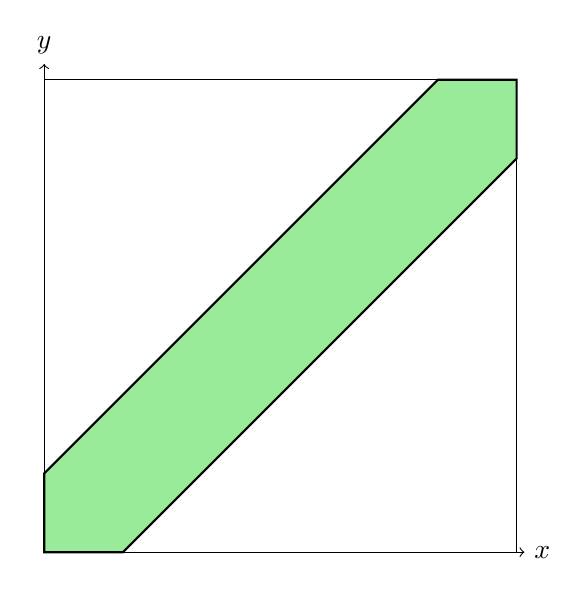
\begin{tikzpicture}
      \draw[->] (0,0) -- (6.1,0) node[right] {$x$};
      \draw[->] (0,0) -- (0,6.2) node[above] {$y$};
      \draw (0,6) -- (6,6) node {};
      \draw (6,0) -- (6,6) node {};
      \draw (0,1) -- (5,6) node {};
      \draw (1,0) -- (6,5) node {};
      \filldraw[thick,fill=green!80!black,fill opacity=0.4] (0,0) -- (1,0) -- (6,5) -- (6,6)  -- (5,6) -- (0,1) -- cycle;
    \end{tikzpicture}
    \caption{Het universum}
  \end{figure}
  Noem $x\in \interval{0}{60}$ de aankomsttijd van de eerste student.
  Noem $y\in \interval{0}{60}$ de aankomsttijd van de tweede student.
  De gebeurtenis waarin de twee studenten elkaar tegenkomen noemen we $A$ en duiden we aan op de grafiek.
  \[ A = \{ (a,b) \mid |a-b| \le 10 \}\]
  We berekenen de gevraagde kans nu als de verhouding van de oppervlakken.
  \[ P(A) = 1 - \frac{\frac{2\cdot 50 \cdot 50 }{2 \cdot}}{60\cdot 60} = \frac{11}{36} \]
\end{oef}

\begin{oef}
  Beschouw een blad met parallelle lijnen op afstand $d$ van elkaar.
  Gooi lukraak een naald van lengte $L$ (veronderstel $L < d$) op het blad.
  Wat is de kans dat de naald minstens \'e\'en van de evenwijdige lijnen snijdt?
  \begin{figure}[H]
    \centering
    \begin{tikzpicture}[scale=2]
      \draw (0,0) -- (3,0);
      \draw (0,2) -- (3,2);
      \draw[<->] (.1,0) -- (.1,2) node[left] {$d$};
      \draw (1,.5) -- (2,2) node[above] {$\frac{L}{2}$};
      \draw (1,1.25) -- (2,1.25);
      \draw[->] (1.75,1.25) arc (0:30:.5cm);
      \draw (1.75,1.30) node[right] {$\alpha$};
    \end{tikzpicture}
  \end{figure}
  We definieren eerst $\Omega$:
  \[ \Omega = \left\{ (a,\alpha) \mid a \in \interval[open right]{0}{d} \wedge \alpha \in \interval[scaled, open right]{-\frac{\pi}{2}}{ \frac{\pi}{2}} \right\} \]
  \begin{figure}[H]
    \centering
    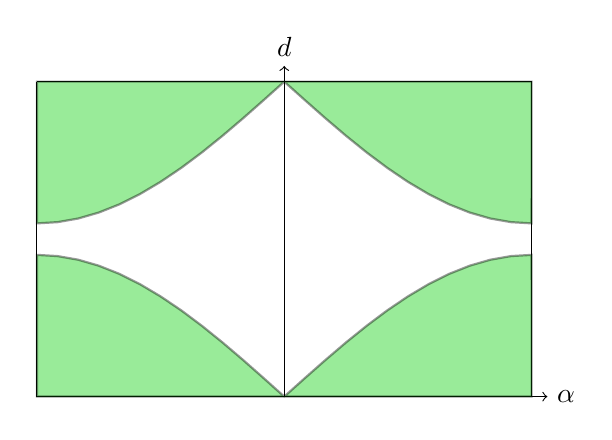
\begin{tikzpicture}[scale=2]
      \draw[->] (-pi/2,0) -- (pi/2+0.1,0) node[right] {$ \alpha $};
      \draw[->] (0,0) -- (0,2.1) node[above] {$d$};
      \draw (-pi/2,0) -- (-pi/2,2) node {};
      \draw (pi/2,0) -- (pi/2,2) node {};
      \draw (-pi/2,2) -- (pi/2,2) node {};
      %\draw[scale=1,domain=-pi/2:pi/2,smooth,variable=\al,red] plot ({\al},{1.8*abs(sin(deg(\al)))});
      %\draw[scale=1,domain=-pi/2:pi/2,smooth,variable=\al,blue] plot ({\al},{1.8-1.8*abs(sin(deg(\al)))});
      \filldraw[thick,fill=green!80!black,opacity=.4] (-pi/2,0) --  plot [domain=-pi/2:pi/2] ({\x},{1.8/2*abs(sin(deg(\x)))}) -- (pi/2,0) -- cycle;
      \filldraw[thick,fill=green!80!black,opacity=.4] (-pi/2,2) --  plot [domain=-pi/2:pi/2] ({\x},{2-1.8/2*abs(sin(deg(\x)))}) -- (pi/2,2) -- cycle;
    \end{tikzpicture}
    \caption{Het universum}
  \end{figure}
  De gebeurtenis dat een naald een lijn overlapt is aangeduid.
  Het is de unie van het deel van het universum waar $a \ge d-\frac{L}{2}\sin(\alpha)$ geldt en het deel waar $a \le \frac{L}{2}\sin(\alpha)$ geldt.
  \[ \left\{ (a,\alpha) \mid (a, \alpha) \in \Omega) \wedge a \ge d-\frac{L}{2}\sin(\alpha) \vee a \le \frac{L}{2}\sin(\alpha) \right\}\]
  We berekenen de oppervlakte van het gekleurde deel dus als volgt:
  \[ 1-2\left(\int_{0}^{\frac{\pi}{2}} d-\frac{L}{2}\sin(\alpha)\ d\alpha- \int_{0}^{\frac{\pi}{2}}\frac{L}{2}\sin(\alpha)\ d\alpha \right) = \frac{2L}{\pi d} \]
\end{oef}

\begin{oef}
  Een vaas bevat $5$ rode en $10$ zwarte ballen.
  Trek lukraak een bal uit de vaas en noteer de kleur.
  Na elke trekking wordt de bal teruggelegd en wordt er \'e\'en extra bal van dezelfde kleur toegevoegd.
  Beantwoord de volgende vragen:
  \begin{itemize}
  \item Gegeven dat de eerste $n$ ballen allemaal zwart zijn, bereken de kans dat de $n+1$-ste bal ook zwart is en bereken de limiet:
    \[ \lim_{n \rightarrow +\infty}P(Z_{n+1}|Z_{1} \cap Z_{2} \cap \dotsb \cap Z_{n}) \]
  \item Gegeven dat de tweede tot en met de $n+1$-ste bal allemaal zwart zijn, bereken de kans dat de eerste getrokken bal zwart was en bereken de limiet:
    \[ \lim_{n \rightarrow +\infty}P(Z_{1}| Z_{2} \cap Z_{3} \cap \dotsb \cap Z_{n+1}) \]
  \end{itemize}
  Voor de trekking zijn er $5$ rode en $10$ en zwarte ballen.
  Wanneer er $r$ rode en $z$ zwarte ballen zijn is de kans $p$ dat er een zwarte bal getrokken word als volgt te berekenen:
  \[ p = \frac{z}{z+r} \]
  \begin{itemize}
  \item  Na $n$ zwarte ballen zijn er $10+n$ zwarte ballen en nog steeds $5$ rode ballen.
    \[ P(Z_{n+1}|Z_{1} \cap Z_{2} \cap \dotsb \cap Z_{n}) = \frac{10+n}{5+10+n} = \frac{10+n}{15+n} \]
    \[ \lim_{n \rightarrow +\infty}P(Z_{n+1}|Z_{1} \cap Z_{2} \cap \dotsb \cap Z_{n}) = \lim_{n \rightarrow +\infty}\frac{10+n}{15+n} = 1 \]
  \item
    Bekijk eerst ook nog de vorige situatie waarbij de eerste bal rood is:
    \[ P(R_{1}) = \frac{5}{15}\]
    \[ P(Z_{2} | R_{1}) = \frac{10}{6+10} \]
    \[ P(Z_{n+1}|R_{1} \cap Z_{2} \cap \dotsb \cap Z_{n}) = \frac{10+(n-1)}{6+10+(n-1)} = \frac{9+n}{15+n} \]
    Gebruik dan zo'n beetje elke rekenregel.
    \[
    \begin{array}{rl}
      P(Z_{1}| Z_{2} \cap Z_{3} \cap \dotsb \cap Z_{n+1})
      &= \frac{P(Z_{1}\cap Z_{2} \cap Z_{3} \cap \dotsb \cap Z_{n+1})}{P(Z_{2} \cap Z_{3} \cap \dotsb \cap Z_{n+1})}\\
      &= \frac{P(Z_{1})P(Z_{2}|Z_{1})P(Z_{3}|Z_{2}\cap Z_{1}) \cdot\ \dotsb\ \cdot P(Z_{n+1}|Z_{1} \cap Z_{2} \cap \dotsb \cap Z_{n}) }{P(Z_{1} \cap Z_{2} \cap Z_{3} \cap \dotsb \cap Z_{n+1})+P(R_{1} \cap Z_{2} \cap Z_{3} \cap \dotsb \cap Z_{n+1})}\\
      &= \frac{\prod_{i=1}^{n}\frac{10+i}{15+i} }{\prod_{i=1}^{n}\frac{10+i}{15+i}+P(R_{1} \cap Z_{2} \cap Z_{3} \cap \dotsb \cap Z_{n+1})}\\
      &= \frac{\prod_{i=1}^{n}\frac{10+i}{15+i} }{\prod_{i=1}^{n}\frac{10+i}{15+i}+\frac{5}{15}\prod_{i=1}^{n}\frac{9+i}{15+i}}\\
      &= \frac{\prod_{i=1}^{n}\frac{10+i}{15+i} }{\frac{10+n}{10}\prod_{i=1}^{n}\frac{9+i}{15+i}+\frac{5}{15}\prod_{i=1}^{n}\frac{9+i}{15+i}}\\
      &= \frac{\frac{10+n}{10}\prod_{i=1}^{n}\frac{9+i}{15+i} }{\left(\frac{10+n}{10}+\frac{5}{15}\right)\prod_{i=1}^{n}\frac{9+i}{15+i}}\\
      &= \frac{\frac{10+n}{10}}{\left(\frac{10+n}{10}+\frac{5}{15}\right)}\\
      &= \frac{10+n}{500+50n}\\
    \end{array}
    \]
    \[ \lim_{n \rightarrow +\infty}P(Z_{n+1}|Z_{1} \cap Z_{2} \cap \dotsb \cap Z_{n}) = \lim_{n \rightarrow +\infty}\frac{10+n}{500+50n} = 1 \]
  \end{itemize}
\end{oef}


\end{document}

%%% Local Variables:
%%% mode: latex
%%% TeX-master: t
%%% End:
